\documentclass{ximera}
\input{../preamble}
\addPrintStyle{..}
\begin{document}
	\author{Wiskunde Op Maat}
	\xmtitle{Complexe getallen voorstelllen in het complexe vlak }{}





\begin{exercise}
\begin{question}
Teken het complexe vlak. Stel het punt \(z = 1 + 2i\) voor in het complexe vlak. 
\end{question}


\begin{hint}

Het complexe vlak is geen 'nieuw' of 'ander' vlak. Als je het complexe vlak tekent, neem je gewoon hetzelfde vlak zoals je dat al kent sinds de lagere school. 
Als je punten in het vlak bekijken als coördinaten of koppels reeële getatten, neem je een horizontale x-as en een verticale y-as. 
Als je punten in het vlak bekijken als complexe getallen, neem je een horizontale reeële-as (met eenheid 1) en een verticale imaginaire-as (met eenheid \(i\)). 

% Vanuit definitie meetkundig 
\begin{image}[0.7\textwidth]
	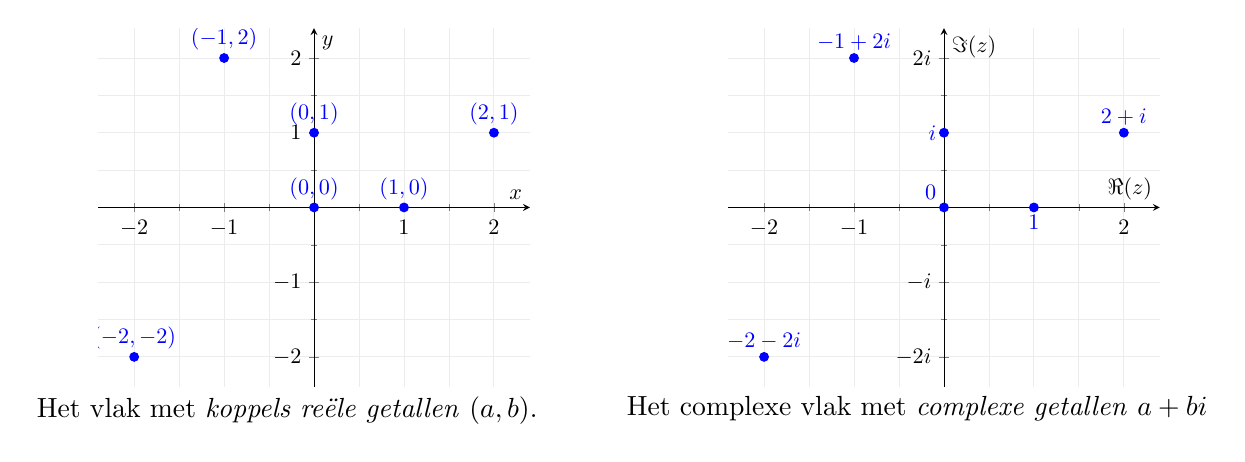
\begin{tikzpicture}[scale=0.8]
		\begin{scope}
			\begin{axis}[
				axis lines = center,
				grid=both,
				grid style={gray!15},
				minor tick num=1,
				% ticks=both,
				xlabel=$x$,
				ylabel=$y$,
				ytick ={-7,...,8}, 
				xtick ={-7,...,8}, 
				ymin=-2,ymax=+2,
				xmin=-2,xmax=+2,
				enlargelimits=true, 
				]
				
				\addplot [blue, mark = *] coordinates {( 0, 0)} node[above] {$(0,0)$};
				\addplot [blue, mark = *] coordinates {( 1, 0)} node[above] {$(1,0)$};
				\addplot [blue, mark = *] coordinates {( 0, 1)} node[above] {$(0,1)$};
				% \addplot [blue, mark = *] coordinates {( 2, 0)} node[above] {$(2,0)$};
				\addplot [blue, mark = *] coordinates {( 2, 1)} node[above] {$(2,1)$};
				\addplot [blue, mark = *] coordinates {( 2,-3)} node[above] {$(2,-3)$};
				\addplot [blue, mark = *] coordinates {(-1, 2)} node[above] {$(-1,2)$};
				\addplot [blue, mark = *] coordinates {(-2,-2)} node[above] {$(-2,-2)$};

			\end{axis}
			\node[below] at (3,0) {Het vlak met \textit{koppels reële getallen} $(a,b)$.};
		\end{scope}

		\begin{scope}[xshift=10cm]
			\begin{axis}[
				axis lines = center,
				grid=both,
				grid style={gray!15},
				minor tick num=1,
				% ticks=both,
				xlabel=$\Re(z)$,
				ylabel=$\Im(z)$,
				ytick ={-7,...,8}, yticklabels={$-7i$, $-6i$, $-5i$, $-4i$, $-3i$, $-2i$, $-i$, $0$, , $2i$, $3i$, $+3i$, $+4i$, $+5i$, $+6i$, $+7i$, $+8i$},
				xtick ={-3,...,3}, xticklabels={$-3$,$-2$,$-1$, , ,$2$,$3$},
				ymin=-2,ymax=+2,
				xmin=-2,xmax=+2,
				enlargelimits=true,
				]
				
				\addplot [blue, mark = *] coordinates {( 0, 0)} node[above left] {$0$};
				\addplot [blue, mark = *] coordinates {( 1, 0)} node[below] {$1$};
				\addplot [blue, mark = *] coordinates {( 0, 1)} node[left] {$i$};
				%\addplot [blue, mark = *] coordinates {( 2, 0)} node[above left] {$2$};
				\addplot [blue, mark = *] coordinates {( 2, 1)} node[above] {$2+i$};
				\addplot [blue, mark = *] coordinates {( 2,-3)} node[above] {$2-3i$};
				\addplot [blue, mark = *] coordinates {(-1, 2)} node[above] {$-1+2i$};
				\addplot [blue, mark = *] coordinates {(-2,-2)} node[above] {$-2-2i$};
			\end{axis}
			\node[below] at (3,0) {Het complexe vlak met \textit{complexe getallen} \(a+bi\)};
		\end{scope}
	\end{tikzpicture}
\end{image}


\end{hint}

\begin{oplossing}

Het complexe getal \(z = 1 + 2i\) heeft als reëel deel \( \Re(z) = \Re(1+2i) = 1\)  en als imaginair deel \( \Im(z) = \Im(1+2i) = 2 \). 

We nemen 1 eenheid op de reële-as en 2 eenheden op de imaginaire as: 

\begin{image}
	\begin{tikzpicture}[>=stealth, scale=1.0]

		% Draw axes
		\draw[->] (-0.5,0) -- (3.0,0) node[right] {\(\mathrm{Re}(z)\)};
		\draw[->] (0,-0.5) -- (0,3.0) node[above] {\(\mathrm{Im}(z)\)};
		
		% Mark the point z = 1 + 2i
		\filldraw (1,2) circle (2pt) node[right] {\(z = 1 + 2i\)};
		
		% Dashed lines to show real and imaginary parts
		\draw[dashed] (1,2) -- (1,0) node[midway,right] {2};
		\draw[dashed] (1,0) -- (0,0) node[midway,below] {1};
		
		% Optionally, draw an arrow from origin to the point
		% \draw[->] (0,0) -- (1,2);
		% You could label the magnitude if you like:
		% \node at (0.5,1.0) {\(\sqrt{1^2 + 2^2} = \sqrt{5}\)};
	
	\end{tikzpicture}
\end{image}

\end{oplossing}

\end{exercise}


\begin{exercise}

	\begin{question}
		De coördinaat van onderstaand complex getal is gelijk aan \(\answer{-2-i}\).
		\begin{tikzpicture}[scale=1]
			% Draw the real and imaginary axes
			\draw[->] (-5,0) -- (3,0) node[right] {$\Re$};
			\draw[->] (0,-4) -- (0,2) node[above] {$\Im$};
		
			% Add tick marks on the real axis
			\foreach \x in {-4,-3,-2,-1,0,1,2} {
				\draw (\x,0.1) -- (\x,-0.1) node[below] {\(\x\)};
			}
		
			% Add tick marks on the imaginary axis
			\foreach \y in {-3,-2,-1,0,1} {
				\draw (0.1,\y) -- (-0.1,\y) node[left] {\(\y\)};
			}
		
			% Mark the complex number z = -2 - i
			\filldraw[red] (-2,-1) circle (2pt) node[below left] {\(z=-2-i\)};
		\end{tikzpicture}
		
	\end{question}
	\begin{hint}
	Bepaal het reëel en imaginair deel van het complex getal. De algemene schrijfwijze van een complex getal is \(z = a+bi\) waarbij \(a = \Re{z}\) en \(b = \Im{z}\).  
	\end{hint}
	\begin{oplossing}

		De algemene schrijfwijze van een complex getal wordt gegeven door \(z = a+bi = \Re{z}+ \Im{z}i\). Het reëel en imaginair deel lezen we af door te projecteren op de assen. 

		\begin{tikzpicture}[scale=1]
			% Draw real and imaginary axes
			\draw[->] (-5,0) -- (3,0) node[right] {$\Re$};
			\draw[->] (0,-4) -- (0,2) node[above] {$\Im$};

			% Tick marks for the real axis
			\foreach \x in {-4,-3,-2,-1,0,1,2} {
				\draw (\x,0.1) -- (\x,-0.1) node[below] {\(\x\)};
			}
			
			% Tick marks for the imaginary axis
			\foreach \y in {-3,-2,-1,0,1} {
				\draw (0.1,\y) -- (-0.1,\y) node[left] {\(\y\)};
			}

			% Mark the complex number z = -2 - i
			\filldraw[red] (-2,-1) circle (2pt) node[below left] {\(z = -2 - i\)};

			% Draw projection to the real axis (vertical dashed line)
			\draw[dashed] (-2,-1) -- (-2,0);
			\node[above] at (-2,0) {\(\Re(z) = -2\)};

			% Draw projection to the imaginary axis (horizontal dashed line)
			\draw[dashed] (-2,-1) -- (0,-1);
			\node[right] at (0,-1) {\(\Im(z) = -1\)};
		\end{tikzpicture}
			
	\end{oplossing}

\end{exercise}	

\begin{exercise}
	Teken volgende complexe getallen in het complexe vlak: 
	\begin{itemize}
		\item \(1\)
		\item \(i\)
		\item \(-1\)
		\item \(-i\)
		\item \(0\)
	\end{itemize}
\end{exercise}

\begin{exercise} Stel de volgende getallen voor in het complexe vlak. 
    \begin{itemize}
    	\item \(z_{1} = 3+2i \)
    	\item \(z_{2} = -3+2i\)
    	\item \(z_{3} = 3 + 4i  \)
    	\item \(z_{4} = 5 - 2i  \)
    	\item \(z_{5} = -1-i \)
    \end{itemize}

	\begin{oplossing}
		\begin{image}
		\begin{tikzpicture}[scale=0.8]
			% Draw the real and imaginary axes
			\draw[->] (-7,0) -- (7,0) node[right] {$\Re$};
			\draw[->] (0,-5) -- (0,5) node[above] {$\Im$};
			
			% Draw tick marks on the real axis
			\foreach \x in {-6,-5,...,6} {
				\draw (\x,0.1) -- (\x,-0.1) node[below] {\(\x\)};
			}
			
			% Draw tick marks on the imaginary axis
			\foreach \y in {-4,-3,...,4} {
				\draw (0.1,\y) -- (-0.1,\y) node[left] {\(\y\)};
			}
			
			% Plot the points
			\filldraw[blue] (3,2) circle (2pt) node[above right] {\(z_{1}=3+2i\)};
			\filldraw[blue] (-3,2) circle (2pt) node[above left] {\(z_{2}=-3+2i\)};
			\filldraw[blue] (3,4) circle (2pt) node[above right] {\(z_{3}=3+4i\)};
			\filldraw[blue] (5,-2) circle (2pt) node[below right] {\(z_{4}=5-2i\)};
			\filldraw[blue] (-1,-1) circle (2pt) node[below left] {\(z_{5}=-1-i\)};
		\end{tikzpicture}
	\end{image}

	\end{oplossing}
    
\end{exercise}



\begin{exercise} Bepaal volgende complexe getallen 
        
\begin{question} \( z_{1} = \answer{-2 + i  } \) \end{question}
\begin{question} \( z_{2} = \answer{0       } \) \end{question}
\begin{question} \( z_{3} = \answer{-1 - 3i } \) \end{question}
\begin{question} \( z_{4} = \answer{-7i     } \) \end{question}
\begin{question} \( z_{5} = \answer{7 + 2i  } \) \end{question}


\begin{image}	
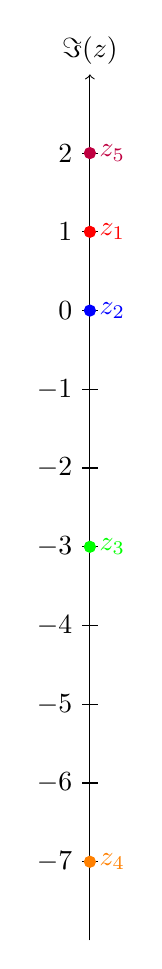
\begin{tikzpicture}[scale=1]
    % Draw the imaginary axis (vertical axis)
    \draw[->] (0,-8) -- (0,3) node[above] {\(\Im(z)\)};
    
    % Add tick marks on the imaginary axis
    \foreach \y in {-7,-6,-5,-4,-3,-2,-1,0,1,2} {
        \draw (0.1,\y) -- (-0.1,\y) node[left] {\(\y\)};
    }
    
    % Plot the points using only their imaginary parts
    \filldraw[red] (0,1) circle (2pt) node[right] {\(z_1\)};
    \filldraw[blue] (0,0) circle (2pt) node[right] {\(z_2\)};
    \filldraw[green] (0,-3) circle (2pt) node[right] {\(z_3\)};
    \filldraw[orange] (0,-7) circle (2pt) node[right] {\(z_4\)};
    \filldraw[purple] (0,2) circle (2pt) node[right] {\(z_5\)};
    
\end{tikzpicture}
\end{image}
    
\end{exercise}





\end{document}